\documentclass[12pt, letterpaper]{article}
\usepackage[utf8]{inputenc}
\usepackage{graphicx}
\usepackage{float}

\graphicspath{{../figures/}}
\begin{document}

\begin{titlepage}
    \begin{center}
        \begin{center}
             
\includegraphics[width=0.5\textwidth]{figures/collegelogo.png}
        \end{center}
        \Large
        K. K. Institute of Engineering Education and Research\\
        Department of Computer Engineering\\
        \vspace{0.5 in}
        \Huge
        \textbf{Project Report}\\
        \vspace*{0.5 in}
        \Large
        \textbf{Data Mining and Warehousing}
        \vspace{1 in}
                
        \Large
        Guided by:                  \hfill                 By: \hspace*{1.35in} \\
        Prof. Jyoti Mankar     \hfill           Shreyas Kalvankar (17)\\
        				\hspace{2.95 in}			 Hrushikesh Pandit(18)\\
        				\hspace{2.8 in}			 Pranav Parwate (19)\\
        				\hspace{2.55 in}			 Atharva Patil (20)\\
        
        \vspace*{1 in}
        
        A.Y. 2020-21 Sem I
    \end{center}
\end{titlepage}


\tableofcontents
\newpage

\section{Problem Statement}

\hspace*{0.25 in}To study, observe and classify the DeepSat-6 Airborne Dataset into 6 categories using Data Mining Algorithms.

\subsection{Objectives}
\begin{itemize}
	\item Study the DeepSat-6 Airborne Dataset with respect to application of Data Mining Algorithms.
	\item Study variations in data using Principle Component Analysis and TSNE.
	\item Perform feature extraction and data classification by using Convolutional Neural Networks.
\end{itemize}

\newpage
\section{Introduction}
\hspace*{0.25 in}Originally, images were extracted from the National Agriculture Imagery Program (NAIP) dataset. The NAIP dataset consists of a total of 330,000 scenes spanning the whole of the Continental United States (CONUS). The authors used the uncompressed digital Ortho quarter quad tiles (DOQQs) which are GeoTIFF images and the area corresponds to the United States Geological Survey (USGS) topographic quadrangles. The average image tiles are ~6000 pixels in width and ~7000 pixels in height, measuring around 200 megabytes each. The entire NAIP dataset for CONUS is ~65 terabytes. The imagery is acquired at a 1-m ground sample distance (GSD) with a horizontal accuracy that lies within six meters of photo-identifiable ground control points.
\hspace*{0.25 in}The images consist of 4 bands - red, green, blue and Near Infrared (NIR).In order to maintain the high variance inherent in the entire NAIP dataset, we sample image patches from a multitude of scenes (a total of 1500 image tiles) covering different landscapes like rural areas, urban areas, densely forested, mountainous terrain, small to large water bodies, agricultural areas, etc. covering the whole state of California.
\newpage
\section{Requirements}
\subsection{Software Requirements}
\begin{center}
\begin{table}[!htb]
		\begin{tabular}{| c | c | c |}
		\hline
		\textbf{Sr. no.} & \textbf{Parameter} & \textbf{Requirement} \\
		\hline
		1 & Operating System & Windows \\
		\hline
		2 &  IDE & Jupyter Notebook \\
		\hline
		3 & Programming Language & Python3 \\
		\hline
		\end{tabular}
		\caption{Software Requirements}

\end{table}
\end{center}


\subsection{Hardware Requirements}

\begin{table}[!htb]
\begin{center}
		\begin{tabular}{| c | c | c | c |}
		\hline
		\textbf{Sr. no.} & \textbf{Parameter} & \textbf{Requirement} & \textbf{Justification}\\
		\hline
		1 & GPU &  Nvidia GeForce GTX 1050 & Training the model \\
		\hline
		2 & GPU Memory & $>$4 GB & Batch Training\\
		\hline
		\end{tabular}
		\caption{Hardware Requirements}
\end{center}
\end{table}

\newpage
\section{Methodology}
\subsection{Algorithm}

\hspace*{0.25 in}Principal component analysis (PCA) is the process of computing the principal components and using them to perform a change of basis on the data, sometimes using only the first few principal components and ignoring the rest.The principal components of a collection of points in a real p-space are a sequence of ${\displaystyle p}$p direction vectors, where the $i^{th}$ vector is the direction of a line that best fits the data while being orthogonal to the first $${\displaystyle i-1}i-1$$ vectors. Here, a best-fitting line is defined as one that minimizes the average squared distance from the points to the line.PCA is used in exploratory data analysis and for making predictive models. It is commonly used for dimensionality reduction by projecting each data point onto only the first few principal components to obtain lower-dimensional data while preserving as much of the data's variation as possible.
First Component:
\begin{center}
             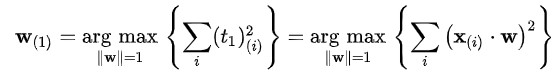
\includegraphics[width=0.5\textwidth]{figures/firstc.jpg}
\end{center}

Further Component :
\begin{center}
             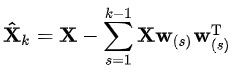
\includegraphics[width=0.5\textwidth]{figures/secondc.jpg}
\end{center}
\newpage
\begin{center}
             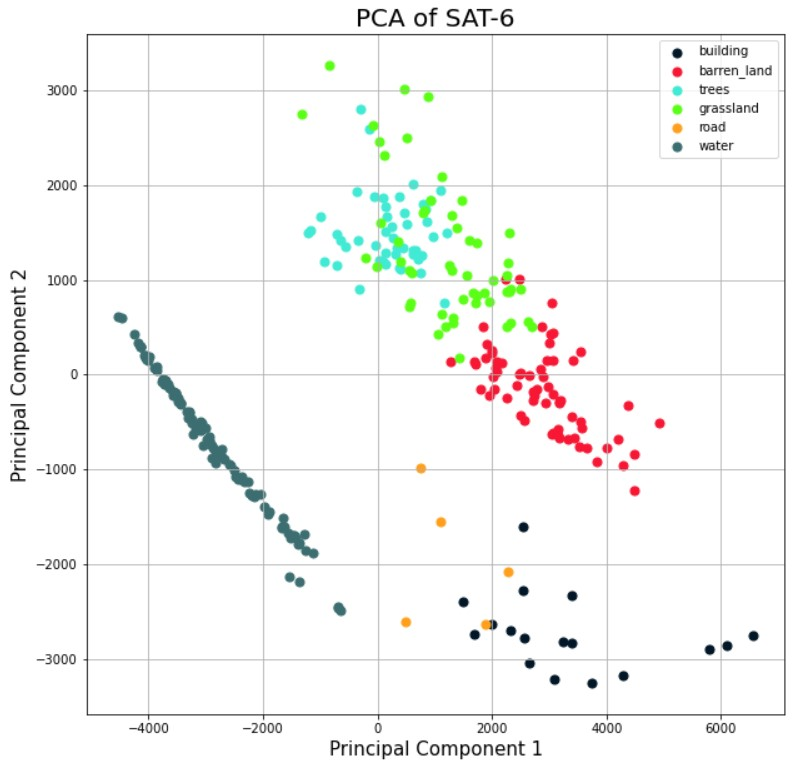
\includegraphics{figures/pca.jpg}
\end{center}
\newpage
\hspace*{0.25 in}t-distributed stochastic neighbor embedding (t-SNE) is a statistical method for visualizing high-dimensional data by giving each datapoint a location in a two or three-dimensional map. It is based on Stochastic Neighbor Embedding originally developed by Sam Roweis and Geoffrey Hinton, where Laurens van der Maaten proposed the t-distributed variant.It is a nonlinear dimensionality reduction technique well-suited for embedding high-dimensional data for visualization in a low-dimensional space of two or three dimensions. Specifically, it models each high-dimensional object by a two- or three-dimensional point in such a way that similar objects are modeled by nearby points and dissimilar objects are modeled by distant points with high probability.The t-SNE algorithm comprises two main stages. First, t-SNE constructs a probability distribution over pairs of high-dimensional objects in such a way that similar objects are assigned a higher probability while dissimilar points are assigned a lower probability.Second, t-SNE defines a similar probability distribution over the points in the low-dimensional map, and it minimizes the Kullback–Leibler divergence (KL divergence) between the two distributions with respect to the locations of the points in the map.
\begin{center}
             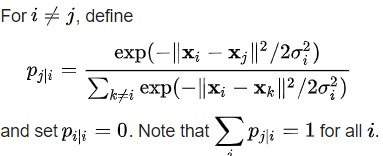
\includegraphics[width=0.5\textwidth]{figures/tsne.jpg}
\end{center}

\newpage
\begin{center}
             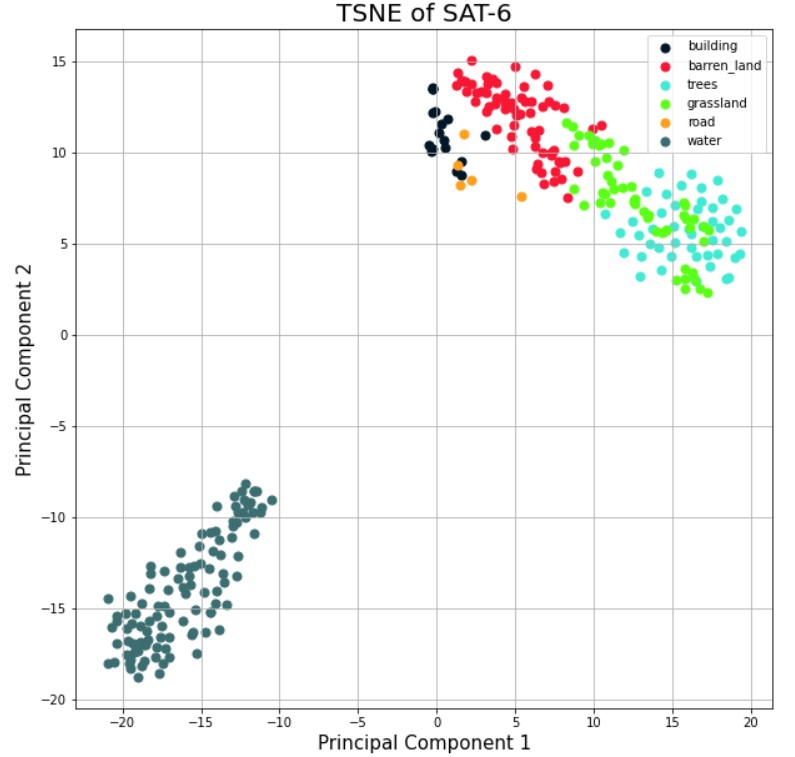
\includegraphics{figures/tsnegraph.jpg}
\end{center}
\newpage
\hspace*{0.25 in}CNNs are regularized versions of multilayer perceptrons. Multilayer perceptrons usually mean fully connected networks, that is, each neuron in one layer is connected to all neurons in the next layer. The "fully-connectedness" of these networks makes them prone to overfitting data. Typical ways of regularization include varying the weights as the loss function gets minimized while randomly trimming connectivity. CNNs take a different approach towards regularization: they take advantage of the hierarchical pattern in data and assemble patterns of increasing complexity using smaller and simpler patterns embossed in the filters. Therefore, on the scale of connectedness and complexity, CNNs are on the lower extreme.
\begin{figure}[!h]
    \centering
    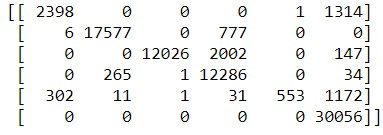
\includegraphics{figures/confuse.jpg}
    \caption{Confusion Matrix}
    \label{Confusion Matrix}
\end{figure}

\newpage
\section{Results}

\begin{center}
    \begin{table}
	\begin{tabular}{ c c c c c}
		& precision & recall & f1-score & support \\
    building    &   0.89 &     0.65  &    0.75   &   3713 \\
barren\_land     &  0.98  &    0.96   &   0.97  &   18360 \\
      trees      & 1.00  &    0.85   &   0.92  &   14175 \\
 grassland      & 0.81  &    0.98   &   0.89   &  12586 \\
      road      & 1.00  &    0.27    &  0.42  &    2070 \\
     water      & 0.92  &    1.00   &   0.96   &  30056 \\

  accuracy       &  ---      &   ---   &      0.93   &  80960 \\
 macro avg      & 0.93    &  0.78 &     0.82  &   80960 \\
weighted avg      & 0.93 &     0.93     & 0.92   &  80960 \\



	\end{tabular}
	\caption{Classification Report}
    \label{Classification Report}
	\end{table}
\end{center}


\newpage

\section{Conclusion}
\hspace*{0.25 in}Thus we have successfully mined the DeepSat - 6 Airborne Dataset using Principle Component Analysis and t-distributed stochastic neighbor embedding (t-SNE).
\end{document}
